\section{Course Pages}
\subsection{Overview}
The course pages are a crucial component of any learning management system. It is the place where students and academics mainly interact with the LMS and acts the centralised page in which other components are linked, for example the lectures, tutorials and quizzes. 
The course pages also includes the course content and course outline pages. The course content is the page where slides, tutorial questions and notes are found and the course outline is where the crucial course outline and learning outcomes of the course are found.
These pages offer other bonus functionality such as widgets which will be discussed in further sections.

\subsection{Pages}
The main 3 pages that the course pages will encompass are:
\begin{itemize}
    \item The main dashboard/page
    \item The course content page
    \item The course outline page
\end{itemize}

\subsubsection{Main Dashboard/Page}
The main dashboard/page is 
\begin{figure}[h]
    \centering
    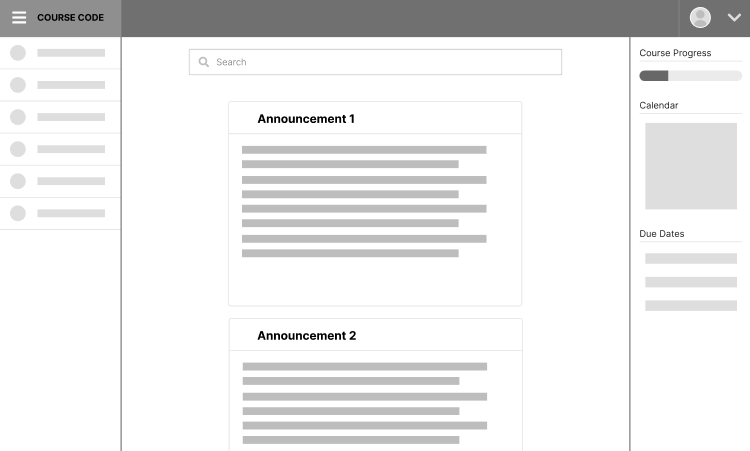
\includegraphics[scale=0.5]{course-pages-main}
    \caption{The main dashboard/page within the course}
\end{figure}
\subsubsection{Course Content Page}
\subsubsection{Course Outline Page}